\documentclass[a4paper,12pt]{article}
\usepackage[spanish,es-tabla]{babel}
\usepackage[margin=25mm]{geometry}
\usepackage[hidelinks]{hyperref}
\usepackage[backend=biber,citestyle=numeric]{biblatex}
\usepackage{lmodern,amsmath,mathptmx,amssymb,amsfonts,enumerate,float,fullpage,graphicx,makeidx,caption,colortbl,xcolor,hhline,tabularx,array,tabularray,booktabs,arydshln,multirow,comment}
\numberwithin{figure}{section}
\numberwithin{equation}{section}
\numberwithin{table}{section}
\renewcommand{\baselinestretch}{1.5}


\bibliography{referencias}
\graphicspath{{imagenes/}}

\begin{document}

\input{portada}

\section{Introducción}

En el presente trabajo se aborda el diseño de una línea de transmisión bifilar, un tipo de conductor eléctrico compuesto por dos hilos paralelos separados por un dieléctrico. Este tipo de línea es ampliamente utilizado en diversas aplicaciones de telecomunicaciones debido a sus características particulares.

El objetivo principal de este estudio es desarrollar un diseño que cumpla con un conjunto específico de requisitos, incluyendo una impedancia característica, una capacitancia por unidad de longitud, una atenuación nominal  y una velocidad de propagación del $98 \%$ de la velocidad de la luz en el vacío.

La importancia de este diseño radica en la necesidad de transmitir señales electromagnéticas de manera eficiente y con mínimas pérdidas en aplicaciones donde estas especificaciones son fundamentales. A través de este trabajo, se busca analizar los factores que influyen en el rendimiento de una línea de transmisión bifilar y proponer una solución óptima que satisfaga los requerimientos establecidos.

En las siguientes secciones se presentarán los fundamentos teóricos de las líneas de transmisión, el procedimiento de diseño seguido y los resultados obtenidos. Finalmente, se discutirán las posibles aplicaciones de este diseño y se propondrán líneas futuras de investigación.


\pagebreak


\section{Problema planteado}
Se desea diseñar una línea de transmisión bifilar, con las siguientes características:

\begin{itemize}
    \item Impedancia Característica: $300 \Omega$.
    \item Capacitancia por unidad de longitud: $10 pF/m$.
    \item Atenuación nominal: $1.9 dB/m$, a $100MHz$.
    \item Velocidad de propagación nominal: $98\%$.
\end{itemize}

Se definirá posteriormente el dieléctrico a utilizar, el tipo de conductor y dimensiones (diámetros de los conductores, separación entre conductores, etc).

\pagebreak

\section{Descripción teórica}

\subsection{Linea de transmisión bifilar}
Una línea de transmisión bifilar es un tipo de conductor eléctrico compuesto por dos hilos paralelos separados por un dieléctrico. Este tipo de línea es ampliamente utilizado en diversas aplicaciones de telecomunicaciones debido a su simplicidad constructiva y sus características de transmisión.

\subsection{Impedancia Característica}

Uno de los parámetros más importantes de una línea de transmisión es la impedancia característica ($Z_o$). Esta representa la relación entre el voltaje y la corriente que se propaga a lo largo de la línea en modo transversal electromagnético (TEM). La impedancia característica de una línea bifilar depende de la geometría de los conductores (diámetros y separación) y de las propiedades del dieléctrico (permitividad relativa).
        \begin{center}
        \begin{figure}[H]
        \centering  
        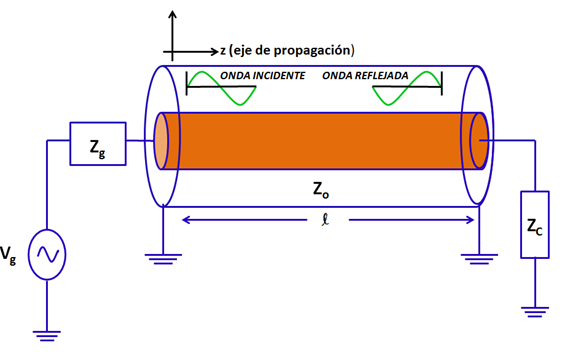
\includegraphics[scale=0.7]{imagenes/Modelo esquemático de una línea de transmisión conectada.png}
        \caption{Modelo esquemático de una línea de transmisión conectada}
        \end{figure}
        \end{center}

\subsection{Velocidad de Propagación}

La velocidad de propagación de una onda electromagnética a lo largo de una línea de transmisión es menor que la velocidad de la luz en el vacío y depende de la permitividad relativa del dieléctrico. Esta velocidad se relaciona con la longitud de onda de la señal y el período de la misma.
        \begin{center}
        \begin{figure}[H]
        \centering  
        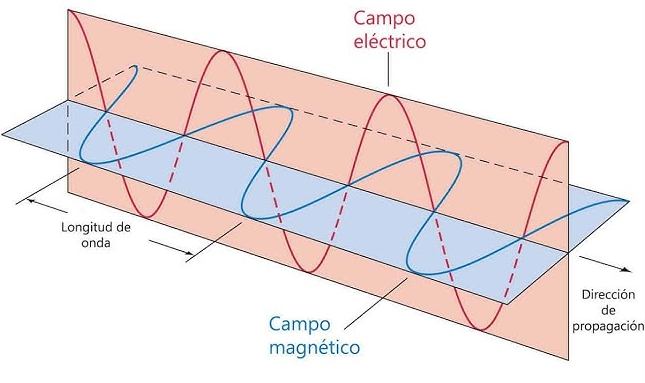
\includegraphics[scale=0.7]{imagenes/propagacion de una onda electromagnetica.png}
        \caption{Propagación de una onda electromagnética}
        \end{figure}
        \end{center}
\subsection{Atenuación}

La atenuación representa la pérdida de potencia de la señal a medida que se propaga a lo largo de la línea. Esta pérdida se debe a varios factores, como la resistencia óhmica de los conductores, las pérdidas dieléctricas y las pérdidas por radiación. La atenuación se expresa en decibelios por unidad de longitud (dB/m).

\subsection{Capacitancia y Inductancia en una linea de transmisión bifilar}

Una línea de transmisión bifilar puede ser modelada como una sucesión infinita de elementos infinitesimales, cada uno compuesto por una inductancia y una capacitancia. La capacitancia se debe a la presencia del campo eléctrico entre los conductores, mientras que la inductancia se debe al campo magnético generado por la corriente que circula por los conductores.

\subsection{Modelo de Línea de Transmisión}

Para analizar el comportamiento de una línea de transmisión, se utiliza el modelo de línea de transmisión distribuida, que considera la distribución continua de los parámetros a lo largo de la línea. Este modelo permite obtener las ecuaciones de telegrafistas, que relacionan el voltaje y la corriente en cualquier punto de la línea.

        \begin{center}
        \begin{figure}[H]
        \centering  
        \includegraphics[scale=1]{imagenes/Modelo de parámetros distribuidos.png}
        \caption{Modelo de parámetros distribuidos}
        \end{figure}
        \end{center}

        \begin{center}
        \begin{figure}[H]
        \centering  
        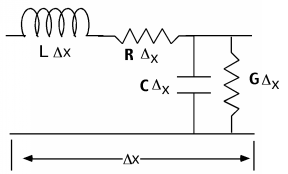
\includegraphics[scale=1]{imagenes/Modelo distribuido completo.png}
        \caption{Modelo distribuido completo}
        \end{figure}
        \end{center}
%\subsetion{Línea bifilar (altas frecuencias)}[\cite{hayt}] %se le agrega [1] según la bibliografia o \cite{nombre}

\begin{comment}Para la línea de transmisión bifilar que muestra la figura \ref{fig:linea-bifilar} con conductores de radio a y
conductividad σc con una separación entre centros igual a d y un medio de permeabilidad μ,

que la capacitancia está dada por \end{comment}

\begin{comment}
\subsection{Relación con el Problema}
permitividad , y conductividad σc, se encontró en el capítulo 6 [ecuación (40), sección 6.5]
En este trabajo, los conceptos teóricos mencionados anteriormente se aplicarán para diseñar una línea de transmisión bifilar que cumpla con las especificaciones establecidas. Se utilizarán las ecuaciones de línea de transmisión para calcular las dimensiones geométricas de la línea y verificar que se obtenga la impedancia característica, la capacitancia y la velocidad de propagación deseadas. Además, se analizarán las pérdidas en la línea para evaluar el cumplimiento de la especificación de atenuación.

Esta sección puede ser ampliada o modificada según tus necesidades. Puedes agregar más detalles sobre los conceptos que consideres relevantes, como:

\textbf{Modos de propagación:} Explicar brevemente los diferentes modos de propagación en líneas de transmisión y por qué se considera el modo TEM en este caso.
\textbf{Coeficiente de reflexión:} Definir el coeficiente de reflexión y su importancia en el diseño de líneas de transmisión.
\textbf{Adaptación de impedancias:} Explicar la importancia de adaptar la impedancia de la línea a la impedancia de la carga para evitar reflexiones.
\end{comment}

\pagebreak


\input{PROPUESTADE DISEÑO y esquemas}

\section{Valores de dispositivos o elementos}
\begin{figure}[H]
    \centering
    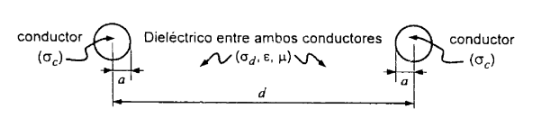
\includegraphics[width=5in]{lineasbifilares.png}
    \caption{Esquema de lineas bifilares}
    \label{fig:EsquemaBifilar}
\end{figure}

\begin{itemize}
    \item C=11 $\frac{pF}{m}$
    \item L=1 $\frac{\mu H}{m}$
    \item G=0 $\frac{S}{m}$
    \item R=0.8 $\Omega$
    \item a= 1mm
    \item d=12mm
    \item $\beta = 2.1386 \frac{rad}{m}$
    \item $\epsilon_r$ = 1,0412 (material del dieléctrico es aire)
    \item  $\sigma_c= 4,8x10^7$
\end{itemize}


\pagebreak

\section{Conclusiones y posibles aplicaciones}

En este trabajo se ha llevado a cabo el diseño de una línea de transmisión bifilar, cumpliendo con las especificaciones establecidas para impedancia característica, capacitancia, atenuación y velocidad de propagación. Se ha obtenido un diseño óptimo que minimiza las pérdidas y maximiza la eficiencia de la transmisión.

Una de las aplicaciones más prometedoras de esta línea de transmisión bifilar es en el campo de las antenas dipolo. Al utilizar esta línea como alimentador de una antena dipolo, se puede lograr una mejor adaptación de impedancias, reduciendo las pérdidas por reflexión y mejorando la eficiencia de radiación. Además, la baja atenuación de la línea permite transmitir señales a mayores distancias sin una degradación significativa de la señal.

El diseño de una línea de transmisión bifilar es un tema de gran relevancia en el campo de las telecomunicaciones. Los resultados obtenidos en este trabajo demuestran la viabilidad de diseñar líneas de transmisión personalizadas para aplicaciones específicas, como las antenas dipolo, antenas de radio, TV, etc.



\pagebreak


\section{Referencias Bibliográficas}

\begin{itemize}
    \item Neri Vela, R. (1999). Líneas de transmisión (1.ª ed.). México: McGraw-Hill.

    \item Hayt, W. H., Jr., \& Buck, J. A. (2006). Teoría electromagnética (7ª ed.). México: McGraw-Hill.
\end{itemize}

\pagebreak
%\section{Bibliografía y}
%\printbibliography

\end{document}
